% The PCB-scale constants of upstream KiCad placed on a logarithmic length
% axis against interposer geometry, and where the fork moves each of them.
\documentclass[border=4pt]{standalone}
\usepackage{tikz}
\usetikzlibrary{arrows.meta, positioning, calc, backgrounds}
\usepackage[T1]{fontenc}
\usepackage{lmodern}

\definecolor{IHPfg}{RGB}{0,80,139}
\definecolor{IHPred}{RGB}{228,15,19}
\definecolor{IHPaccent}{RGB}{109,112,114}
\definecolor{IHPgreen}{RGB}{65,155,75}

\begin{document}
% x is one decade of length, starting at 1 nm; y is centimetres.
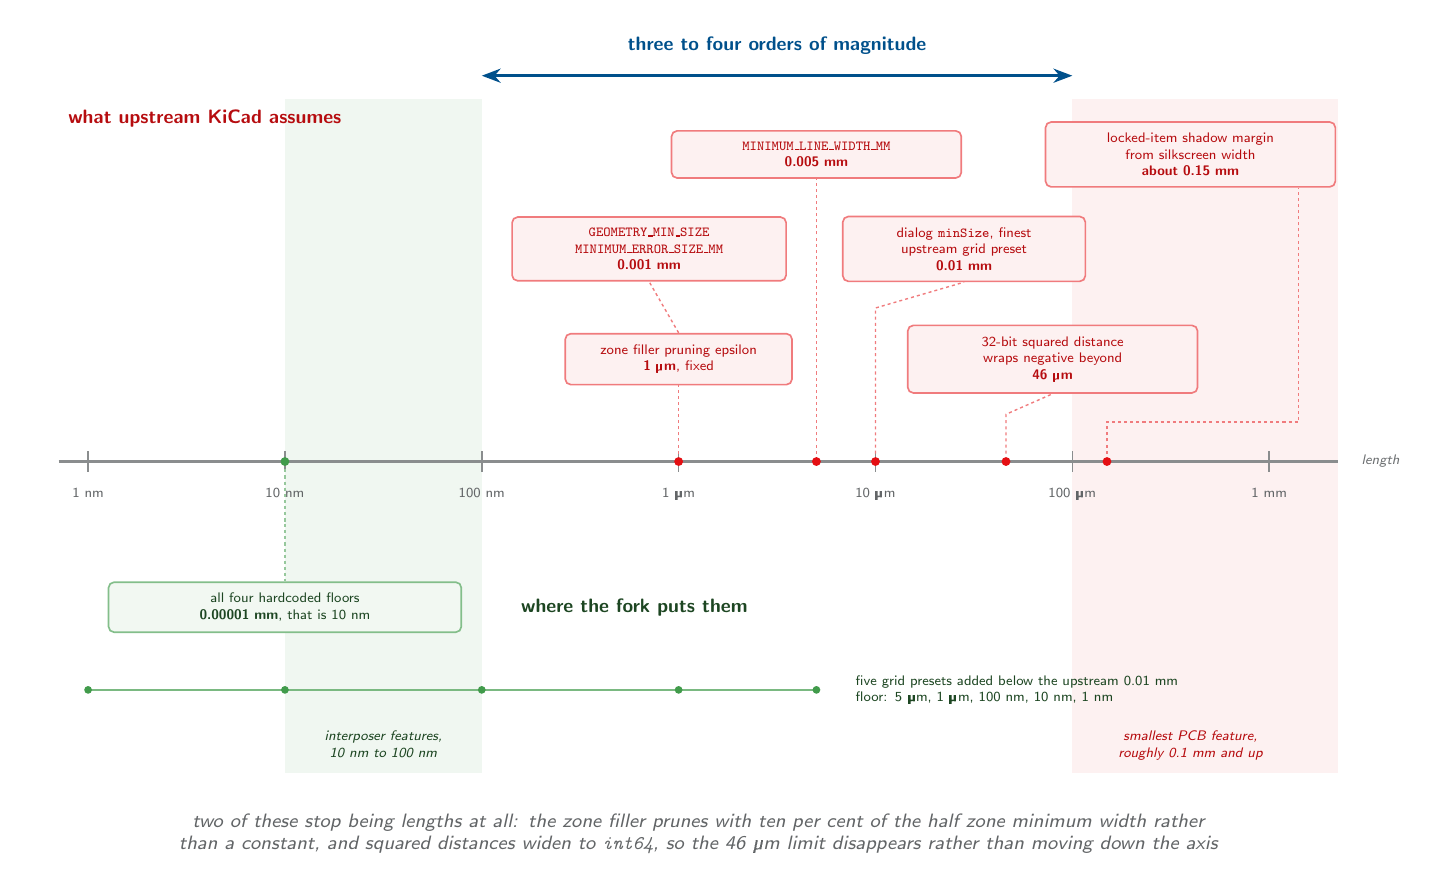
\begin{tikzpicture}[
    x=2.5cm, y=1cm, >=Stealth,
    upbox/.style={
        rectangle, rounded corners=2pt,
        draw=IHPred!55, fill=IHPred!6, line width=0.6pt,
        text width=#1, inner sep=1.4mm,
        font=\sffamily\tiny, text=IHPred!80!black, align=center
    },
    downbox/.style={
        rectangle, rounded corners=2pt,
        draw=IHPgreen!65, fill=IHPgreen!7, line width=0.6pt,
        text width=#1, inner sep=1.4mm,
        font=\sffamily\tiny, text=IHPgreen!45!black, align=center
    },
    lead/.style={
        line width=0.5pt, color=#1!55, dash pattern=on 1.1pt off 1.1pt
    },
    ticklbl/.style={font=\sffamily\tiny, text=IHPaccent!90!black},
    bandlbl/.style={font=\sffamily\tiny\itshape, align=center},
    colhead/.style={font=\sffamily\scriptsize\bfseries},
    foot/.style={
        font=\sffamily\scriptsize\itshape, text=IHPaccent!90!black,
        text width=168mm, align=center
    }
]

\coordinate (rmargin) at (6.15, 0);

% =====================================================================
% BANDS: the two design points
% =====================================================================
\begin{pgfonlayer}{background}
    \fill[IHPgreen!8] (1, -3.95) rectangle (2, 4.6);
    \fill[IHPred!6]   (5, -3.95) rectangle (6.35, 4.6);
\end{pgfonlayer}

\node[bandlbl, text=IHPgreen!45!black, text width=30mm, anchor=north]
    at (1.5, -3.3) {interposer features,\\10 nm to 100 nm};
\node[bandlbl, text=IHPred!80!black, text width=32mm, anchor=north]
    at (5.6, -3.3) {smallest PCB feature,\\roughly 0.1 mm and up};

% =====================================================================
% THE GAP
% =====================================================================
\draw[{Stealth[length=2.4mm]}-{Stealth[length=2.4mm]}, line width=0.9pt,
      color=IHPfg] (2, 4.9) -- (5, 4.9);
\node[colhead, text=IHPfg, anchor=south]
    at (3.5, 5.05) {three to four orders of magnitude};

% =====================================================================
% THE AXIS
% =====================================================================
\draw[line width=0.9pt, color=IHPaccent!80] (-0.15, 0) -- (6.35, 0);
\foreach \d/\lab in {0/{1 nm}, 1/{10 nm}, 2/{100 nm}, 3/{1 \textmu m},
                     4/{10 \textmu m}, 5/{100 \textmu m}, 6/{1 mm}} {
    \draw[line width=0.6pt, color=IHPaccent!80] (\d, -0.13) -- (\d, 0.13);
    \node[ticklbl, anchor=north] at (\d, -0.22) {\lab};
}
\node[font=\sffamily\tiny\itshape, text=IHPaccent, anchor=west]
    at (6.42, 0) {length};

% =====================================================================
% ABOVE THE AXIS: the PCB-scale constants upstream ships
% =====================================================================
\node[colhead, text=IHPred!80!black, anchor=west]
    at (-0.15, 4.35) {what upstream KiCad assumes};

% zone filler pruning epsilon, 1 um
\fill[IHPred] (3, 0) circle (1.6pt);
\node[upbox=26mm] (zone) at (3, 1.3)
    {zone filler pruning epsilon\\\textbf{1 \textmu m}, fixed};
\draw[lead=IHPred] (3, 0.1) -- (zone.south);

% GEOMETRY_MIN_SIZE and MINIMUM_ERROR_SIZE_MM, 0.001 mm
\node[upbox=32mm] (geo) at (2.85, 2.7)
    {\texttt{GEOMETRY\_MIN\_SIZE}\\\texttt{MINIMUM\_ERROR\_SIZE\_MM}\\
     \textbf{0.001 mm}};
\draw[lead=IHPred] (zone.north) -- (geo.south);

% dialog minSize and the finest upstream grid, 0.01 mm
\fill[IHPred] (4, 0) circle (1.6pt);
\node[upbox=28mm] (dlg) at (4.45, 2.7)
    {dialog \texttt{minSize}, finest\\upstream grid preset\\\textbf{0.01 mm}};
\draw[lead=IHPred] (4, 0.1) -- (4, 1.95) -- (dlg.south);

% int32 squared-distance limit, 46 um
\fill[IHPred] (4.663, 0) circle (1.6pt);
\node[upbox=34mm] (int32) at (4.9, 1.3)
    {32-bit squared distance\\wraps negative beyond\\\textbf{46 \textmu m}};
\draw[lead=IHPred] (4.663, 0.1) -- (4.663, 0.6) -- (int32.south);

% MINIMUM_LINE_WIDTH_MM, 0.005 mm
\fill[IHPred] (3.7, 0) circle (1.6pt);
\node[upbox=34mm] (linew) at (3.7, 3.9)
    {\texttt{MINIMUM\_LINE\_WIDTH\_MM}\\\textbf{0.005 mm}};
\draw[lead=IHPred] (3.7, 0.1) -- (linew.south);

% locked-item shadow margin, about 0.15 mm
\fill[IHPred] (5.176, 0) circle (1.6pt);
\node[upbox=34mm] (shadow) at (5.6, 3.9)
    {locked-item shadow margin\\from silkscreen width\\\textbf{about 0.15 mm}};
\draw[lead=IHPred] (5.176, 0.1) -- (5.176, 0.5) -- (6.15, 0.5)
    -- (shadow.south -| rmargin);

% =====================================================================
% BELOW THE AXIS: where the fork puts them
% =====================================================================
\node[colhead, text=IHPgreen!45!black, anchor=west]
    at (2.15, -1.85) {where the fork puts them};

\fill[IHPgreen] (1, 0) circle (1.6pt);
\node[downbox=42mm] (floors) at (1, -1.85)
    {all four hardcoded floors\\\textbf{0.00001 mm}, that is 10 nm};
\draw[lead=IHPgreen] (1, -0.1) -- (1, -0.75) -- (floors.north);

\draw[line width=0.7pt, color=IHPgreen!70] (0, -2.9) -- (3.7, -2.9);
\foreach \d in {0, 1, 2, 3, 3.7} {
    \fill[IHPgreen] (\d, -2.9) circle (1.4pt);
}
\node[font=\sffamily\tiny, text=IHPgreen!45!black, text width=44mm,
      align=left, anchor=west]
    at (3.85, -2.9) {five grid presets added below the upstream 0.01 mm
     floor: 5 \textmu m, 1 \textmu m, 100 nm, 10 nm, 1 nm};

% =====================================================================
% FOOTER
% =====================================================================
\node[foot, anchor=north] at (3.1, -4.35)
    {two of these stop being lengths at all: the zone filler prunes with ten per
     cent of the half zone minimum width rather than a constant, and squared
     distances widen to \texttt{int64}, so the 46 \textmu m limit disappears
     rather than moving down the axis};

\end{tikzpicture}
\end{document}
